\documentclass[border=8pt]{standalone}
\usepackage[T1]{fontenc}
\usepackage[utf8]{inputenc}
\usepackage{tikz}
\usetikzlibrary{calc, positioning, fit, backgrounds}
\usepackage{xcolor}
\usepackage{amssymb}

\definecolor{tpcolor}{HTML}{2CA02C}
\definecolor{fpcolor}{HTML}{D62728}
\definecolor{fncolor}{HTML}{FF7F0E}
\definecolor{cardgray}{HTML}{F5F5F5}
\definecolor{rulebox}{HTML}{FFF8E1}
\definecolor{headerblue}{HTML}{1F4E79}

\newcommand{\explcard}[9]{%
  % #1=x, #2=y, #3=type label, #4=type color, #5=site, #6=obs/dt/llm, #7=DT path, #8=top rules, #9=predictors
  \begin{scope}[shift={(#1,#2)}]
    % Card background
    \fill[cardgray, rounded corners=4pt] (0,0) rectangle (7.8,-4.8);
    \draw[#4, thick, rounded corners=4pt] (0,0) rectangle (7.8,-4.8);
    % Header
    \fill[#4, rounded corners=4pt] (0,0) rectangle (7.8,-0.55);
    \node[white, font=\bfseries\small, anchor=west] at (0.2,-0.28) {#3};
    \node[white, font=\small, anchor=east] at (7.6,-0.28) {#5};
    % Content
    \node[font=\footnotesize, anchor=north west, text width=7.4cm] at (0.2,-0.75) {#6};
    % DT path
    \node[font=\footnotesize, anchor=north west, text width=7.4cm] at (0.2,-1.55) {%
      \textbf{DT path:} #7};
    % Predictors
    \node[font=\footnotesize, anchor=north west, text width=7.4cm, text=gray!70!black] at (0.2,-2.2) {#9};
    % Rules box
    \fill[rulebox, rounded corners=2pt] (0.15,-2.85) rectangle (7.65,-4.65);
    \draw[orange!50!brown, rounded corners=2pt] (0.15,-2.85) rectangle (7.65,-4.65);
    \node[font=\footnotesize, anchor=north west, text width=7.2cm] at (0.3,-2.95) {%
      \textbf{Top activated LLM rules:}\\[2pt]
      #8};
  \end{scope}
}

\begin{document}
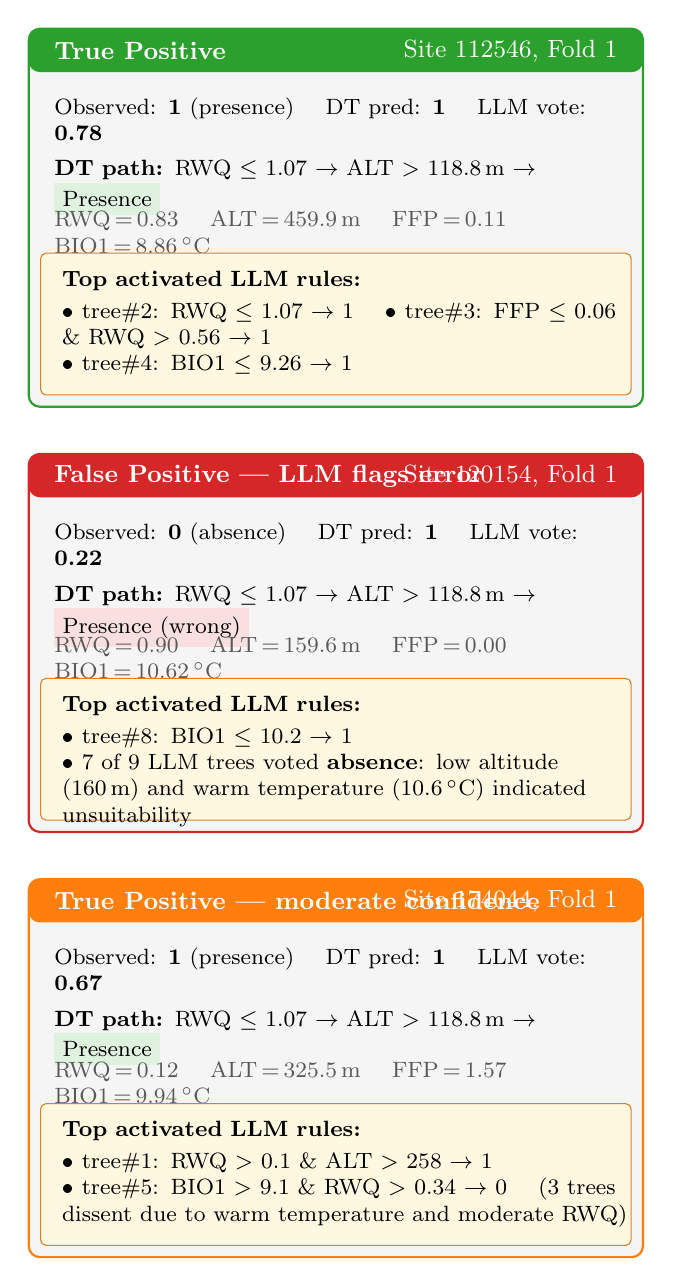
\begin{tikzpicture}

% Card 1: True Positive — site 112546
\explcard{0}{0}%
  {True Positive}{tpcolor}%
  {Site 112546, Fold 1}%
  {Observed: \textbf{1} (presence) \quad DT pred: \textbf{1} \quad LLM vote: \textbf{0.78}}%
  {RWQ $\leq$ 1.07 $\to$ ALT $>$ 118.8\,m $\to$ \colorbox{tpcolor!15}{Presence}}%
  {\footnotesize%
    \textbullet~tree\#2: RWQ $\leq$ 1.07 $\to$ 1 \quad
    \textbullet~tree\#3: FFP $\leq$ 0.06 \& RWQ $>$ 0.56 $\to$ 1\\
    \textbullet~tree\#4: BIO1 $\leq$ 9.26 $\to$ 1}%
  {RWQ\,=\,0.83 \quad ALT\,=\,459.9\,m \quad FFP\,=\,0.11 \quad BIO1\,=\,8.86\,$^\circ$C}

% Card 2: FP where LLM disagrees — site 120154
\explcard{0}{-5.4}%
  {False Positive --- LLM flags error}{fpcolor}%
  {Site 120154, Fold 1}%
  {Observed: \textbf{0} (absence) \quad DT pred: \textbf{1} \quad LLM vote: \textbf{0.22}}%
  {RWQ $\leq$ 1.07 $\to$ ALT $>$ 118.8\,m $\to$ \colorbox{fpcolor!15}{Presence (wrong)}}%
  {\footnotesize%
    \textbullet~tree\#8: BIO1 $\leq$ 10.2 $\to$ 1\\
    \textbullet~7 of 9 LLM trees voted \textbf{absence}: low altitude (160\,m) and warm temperature (10.6\,$^\circ$C) indicated unsuitability}%
  {RWQ\,=\,0.90 \quad ALT\,=\,159.6\,m \quad FFP\,=\,0.00 \quad BIO1\,=\,10.62\,$^\circ$C}

% Card 3: True Positive with moderate LLM — site 174044
\explcard{0}{-10.8}%
  {True Positive --- moderate confidence}{fncolor}%
  {Site 174044, Fold 1}%
  {Observed: \textbf{1} (presence) \quad DT pred: \textbf{1} \quad LLM vote: \textbf{0.67}}%
  {RWQ $\leq$ 1.07 $\to$ ALT $>$ 118.8\,m $\to$ \colorbox{tpcolor!15}{Presence}}%
  {\footnotesize%
    \textbullet~tree\#1: RWQ $>$ 0.1 \& ALT $>$ 258 $\to$ 1\\
    \textbullet~tree\#5: BIO1 $>$ 9.1 \& RWQ $>$ 0.34 $\to$ 0 \quad (3 trees dissent due to warm temperature and moderate RWQ)}%
  {RWQ\,=\,0.12 \quad ALT\,=\,325.5\,m \quad FFP\,=\,1.57 \quad BIO1\,=\,9.94\,$^\circ$C}

\end{tikzpicture}
\end{document}
